%----------------------------------------------------------------
%
%  File    :  thesis-tech.tex
%
%  Author  :  Keith Andrews, IICM, TU Graz, Austria
% 
%  Created :  27 May 93
% 
%  Changed :  19 Feb 2004
% 
%----------------------------------------------------------------


\chapter{Technical Realisation}

\label{chap:Tech}


\chapquote{
Unless you have a deep passion for reformatting, do not even contemplate
writing anything longer than a letter with Microsoft Word.
}
{
Keith Andrews, 2004.
}



Use \LaTeXe\ to produce your thesis. Do \emph{not} even entertain the
idea of writing your thesis with Microsoft Word. Ever.



\section{LaTeX}

\LaTeXe\ provides very comfortable features for structuring and
reorganising your work. In particular, figure and section numbers are
symbolic references and are automatically kept consistent. Even more
importantly, when material is added or changed, \LaTeXe\ reformats
your work \emph{automatically}.

Furthermore, the Biblatex package lets you maintain a database of
bibliographic entries; citations are then also made by symbolic
reference. The exact appearance of citations and the bibliography is
controlled by setting a particular bibliographic style.
See \textcite{WordProcessors} for plenty more reasons to use \LaTeXe\
rather than Word.



\subsection{Literature and Online Resources}

The best reference book for \LaTeXe\ is \textcite{KopkaDaly} -- buy it!
Your advisor can become very irritated by students repeatedly asking
the same basic questions instead of consulting the book.
%
Good online resources for \LaTeXe\ include the Wikibook LaTeX
\parencite{Wikibooks-latex}, \textcite{NotShortIntroLaTeX},
\textcite{FormattingInformation}, the TeX Users Group \parencite{TUG} (see
Figure~\ref{fig:TUG}), and the Deutschsprachige Anwendervereinigung
DANTE \parencite{DANTE} (in German).
%
\LaTeXe\ information in German is available on the local LaTeX@TUG web
site \parencite{LatexTUGraz}. Questions can be asked in the local TU Graz
newsgroup \news{tu-graz.latex}.



\begin{figure}[tp]
\centering
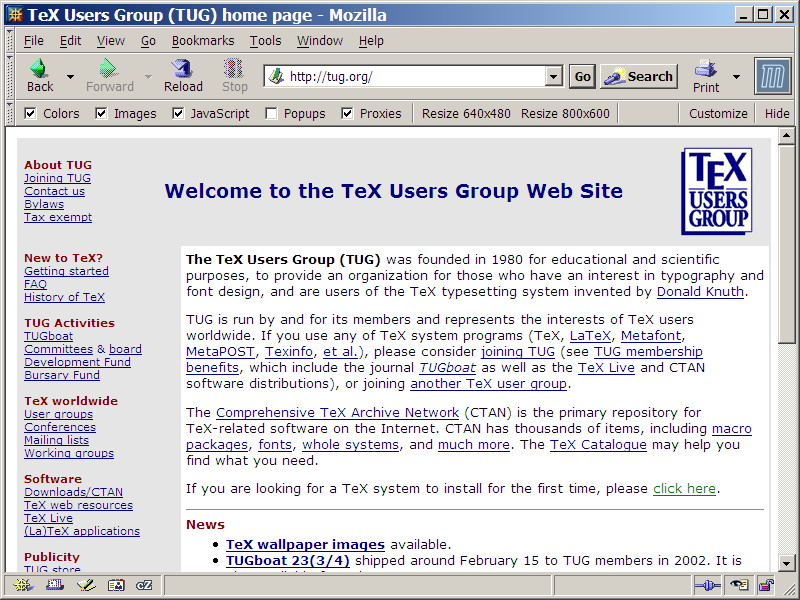
\includegraphics[keepaspectratio,width=\linewidth,height=\halfh]
{images/tugorg.png}

\caption[TeX Users Group web site]{
The web site of the TeX Users Group \parencite{TUG}.
\imgcredit{Screenshot taken by the author of this thesis.}
}
\label{fig:TUG}
\end{figure}




\subsection{Installing \protect\LaTeXe}

For information about availability, versions, installation, etc. of
\LaTeXe\ consult the online
\emph{TeX Frequently Asked Questions} \parencite{TeXfaq}.
%
The best way to install \LaTeXe\ under Windows is to get the latest
TeXLive \parencite{texlive} distribution. You can download an ISO
image from CTAN TeXLive \parencite{ctan-texlive}.  Under Windows 10,
you can mount an ISO image by double-clicking, it is no longer
necessary to actually burn the image to a DVD.





\subsection{Installing Extra \protect\LaTeXe Packages}

Depending on the \LaTeXe\ package you install, you may need to install
additional or more recent versions of \LaTeXe\ packages. For example,
this thesis makes use of the \LaTeXe\ \fname{titlesec} package.
%
You can find a list of packages at your local CTAN site \parencite{CTAN}.
To install a package, read the advice at
\url{http://www.ctan.org/installationadvice/}





\subsection{Running \protect\LaTeXe}

When running \LaTeXe\ under Unix, check that the environment variables
are set to something like the values shown here:
\begin{samepage}
\begin{lstlisting}
setenv TEXINPUTS .:~/tex/inputs:./inputs::
setenv BSTINPUTS .:~/tex/inputs::
setenv BIBINPUTS .:~/tex/bib:./bib::
\end{lstlisting}
\end{samepage}


\LaTeXe\ updates certain auxiliary files during translation (for
example with figure numbers or captions) and makes use of them in
subsequent runs. To be absolutely certain that all references are
resolved correctly, run \fname{pdflatex}, \fname{biber},
\fname{pdflatex}, and \fname{pdflatex} in sequence, as shown
below for this thesis:
\begin{samepage}
\begin{lstlisting}
pdflatex thesis
biber thesis
pdflatex thesis
pdflatex thesis
\end{lstlisting}
\end{samepage}




An alternative is to use the \fname{latexmk} perl script:
\begin{samepage}
\begin{lstlisting}
latexmk --pdf thesis
\end{lstlisting}
\end{samepage}


\fname{latexmk} can also be configured using a config file such as
\lstinline|$HOME/.latexmkrc| in the user's home directory: % dummy comment $
\begin{samepage}
\begin{lstlisting}[language=Perl,]
$pdf_mode = 1;  # force use of pdflatex
\end{lstlisting}   % dummy comment $
\end{samepage}


% latexmk
% http://www.ctan.org/pkg/latexmk/
% http://users.phys.psu.edu/~collins/software/latexmk-jcc/
% http://users.phys.psu.edu/~collins/software/latexmk-jcc/latexmk-437.pdf




\subsection{Spell Checking}

GNU Aspell \parencite{Aspell} is a free open source spell checker.  It can
automatically ignore \LaTeXe\ commands. Aspell can either be run from
the command line or integrated into other packages such as Emacs.





\subsection{Integrated Development Environments (IDEs) for \protect\LaTeXe}

Under Windows you might want to use an integrated development
environment (a fancy editor) for \LaTeXe, which have built-in support
for editing \LaTeXe, spell checking, compiling, and so forth.
The IDEs assume that you have a working \LaTeXe installation,
so install \LaTeXe first.
%
The best are Texmaker \parencite{texmaker}, TeXnicCenter
\parencite{TeXnicCenter} (shown in Figure~\ref{fig:TeXnicCenter}), and LEd
\parencite{LEd}, all of which are free. The shareware WinEdt
\parencite{WinEdt} is also very good.


\begin{figure}[tp]
\centering
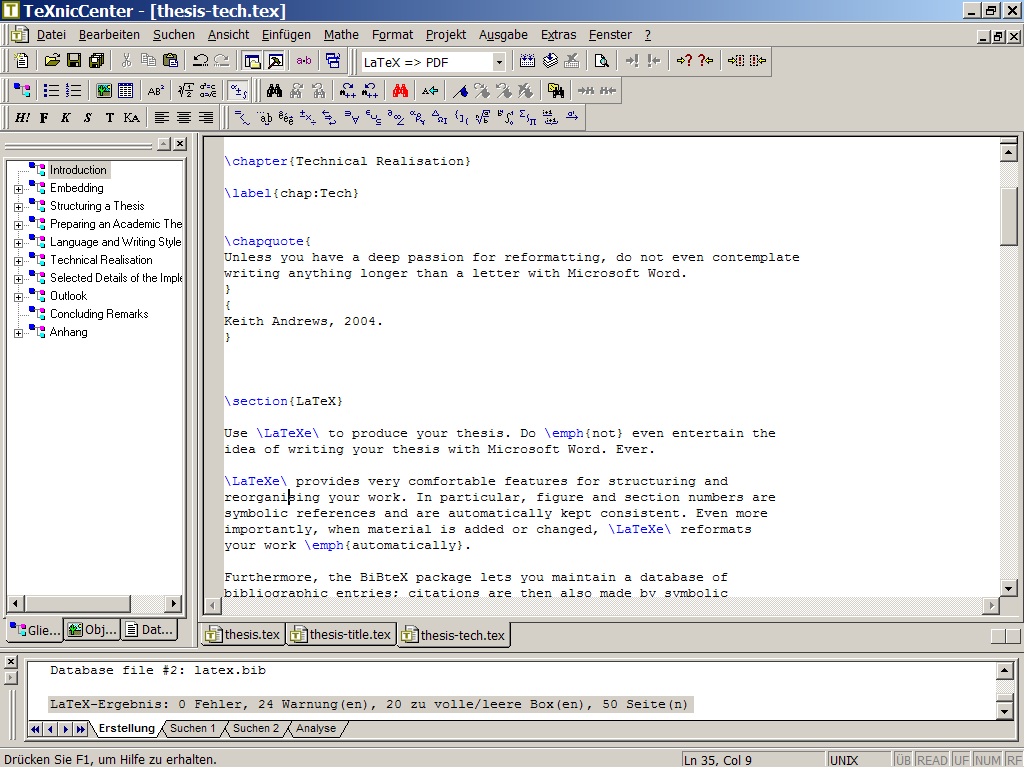
\includegraphics[keepaspectratio,width=\linewidth,height=\halfh]
{images/texnic.png}

\caption[The TeXnicCenter IDE]{
The TeXnicCenter \parencite{TeXnicCenter} integrated development
environment (IDE) for \LaTeXe.
\imgcredit{Screenshot taken by the author of this thesis.}
}
\label{fig:TeXnicCenter}
\end{figure}








\section{Including Images}

Use the \fname{graphicx} package to include images:
\begin{samepage}
\begin{lstlisting}
\usepackage{graphicx}
\end{lstlisting}
\end{samepage}



\subsection{Screenshots}

Screenshots should be made using software such as IrfanView or Gimp
and \emph{saved as PNG}. PNG is a lossless image format which
preserves every pixel of the original image. Sometimes, novices save
screenshots as JPEG (\fname{.jpg}), which is an inherently lossy image
format. Screenshots saved as JPEG invariably introduce artefacts such
as smudged lines and text, due to the way that JPEG achieves its high
compression rates.




\subsection{Diagrams}

Diagrams and illustrations should be drawn using a \emph{vector}
graphics editor such as Adobe Illustrator or
Inkscape\parencite{Inkscape}. Archive (and hand-in) the respective source
files (\fname{.ai} or \fname{.svg}). Convert or export the diagram to
vector PDF for inclusion into \LaTeXe.

Vector graphics are based on objects such as lines, circles, polygons,
and text strings and as such are freely scalable without loss of
quality. In contrast, \emph{raster} graphics are based on pixels and
do not scale without loss of quality. Saving diagrams in a raster
format such as PNG, GIF, or JPEG means they cannot be resized without
considerable loss of quality.





\subsection{Graphs and Plots}

Tabular data can be plotted as, say, a line chart or bar chart, using
the free packages \fname{gnuplot} \parencite{gnuplot} or R \parencite{R-Project}.
The plots should be created as SVG (vector graphics), which can then
be touched up, cropped, and converted to PDF using Adobe Illustrator
or Inkscape\parencite{Inkscape}.





\section{Including Listings}

Use the \vname{listings} package to include source code listings.
There are three types of listing:
\begin{itemize}
\item \liintro{Inline}: A small snippet of code can be contained
  within the flow of a paragraph using \lstinline!\lstinline!, for
  example \lstinline|\lstinline!var i:integer;!| produces
  \lstinline!var i:integer;!.

\item \liintro{In-Place Displayed}: An in-place displayed listing is a
  block of code listed at the place where it occurs. Use in-place
  displayed listings for short blocks of source code upto max $n$
  lines (I use $n=4$). Create an in-place displayed listing with the
  \vname{lstlisting} environment, but without using the \vname{float}
  parameter.

\item \liintro{Floating}: A floating listing is a block of code
  treated like other \LaTeXe floats (such as figures or tables). Use
  floating listings for longer blocks of code. \LaTeXe places the
  listing at some point later on. Create a floating listing with the
  \vname{lstlisting} environment, but specify the \vname{float} and
  \vname{caption} parameters. A floating listing is given a number
  (like Listing 2.1) and is listed in the List of Listings.

\end{itemize}

The \vname{listings} package is currently not designed for use with
UTF8 characters. To use UTF8 characters inside listings, you have to
specify the parameter \lstinline!inputencoding=utf8! and 
specify each character inside the \lstinline!literate=! parameter
to the \lstinline!\lstset! command.








\section{Biblatex and Biber}

BibLaTeX \parencite{BibLaTeX} is a companion system to \LaTeXe, which
allows you to manage sets of references in plain text files (called
\fname{.bib} files) and cite references from within your
\LaTeXe\ documents.  Biber \parencite{Biber} is a program which takes
\fname{.bib} files and manages the formatting of citations and of the
bibliography itself. BibLaTeX and Biber have replaced the now obsolete
BibTeX \parencite{BibTeX}.

